\documentclass[12pt,fleqn]{article}
\setlength{\parindent}{0pt}
\usepackage{graphicx}
\usepackage{cancel}
\usepackage{listings}
\usepackage[latin5]{inputenc}
\usepackage{color}
\setlength{\parskip}{8pt}
\setlength{\parsep}{0pt}
\setlength{\headsep}{0pt}
\setlength{\topskip}{0pt}
\setlength{\topmargin}{0pt}
\setlength{\topsep}{0pt}
\setlength{\partopsep}{0pt}
\setlength{\mathindent}{0cm}
\usepackage{latexsym}
\usepackage{amsfonts}
\usepackage{showkeys}
\renewcommand*\showkeyslabelformat[1]{(#1)}

\begin{document}
Ders 2

Sureklilik

Tanim

$S \subset \mathbb{R}$, $f: S \to \mathbb{R}$ bir fonksiyon olsun, ve $c
\in S$ bir sayi olsun. 
``$f$'in $c$'de surekli oldugu'' soylenir, su durumda: Eger her
$\epsilon>0$ icin bir $\delta > 0$ var ise, oyle ki ne zaman $x \in S$ ve $|x-c| < \delta$
ise, o zaman $|f(x) - f(c)| < \epsilon$ dogrudur. 

Eger  $f: S \to \mathbb{R}$ her $c \in S$ icin dogru ise, yani bir $c$
noktasi degil tum $c$'ler icin gecerli ise, o zaman $f$'in surekli oldugunu
soyleriz. Yani nokta belirtmeye ihtiyac kalmaz. 

Ustteki tanim Analizde dogru anlasilmasi gereken en onemli teorilerden
biridir, ve anlamasi pek kolay degildir. Dikkat edilirse $\delta$ hem
$\epsilon$'a hem de $c$'ye baglidir. Yani her $c \in S$ icin ayni $\delta$
secmemek gerekir. 

Surekli fonksiyon taniminin limitlerin tanimina benziyor olmasi bir
raslanti degil, surekli fonksiyonlarin onemli bir ozelligi zaten onlarin
duzgun limitleri olan kurgular olmalaridir. 

Lipschitz Surekliligi 

Tanim 

$f: S \to \mathbb{R}$ oldugunu kabul edelim, ve oyle bir $K$ sayisi olsun ki $S$
icindeki her $x$ ve$y$ icin 

\[ |f(x) - f(y)| \le K|x-y| \]

ifadesi dogru olsun. O zaman $f$'in ``Lipschitz Surekli'' oldugu soylenir. 

Cok genis bir fonksiyon kategorisi Lipschitz sureklidir. 

Teori 

Bir Lipschitz surekli fonksiyon tutarli / ayni / esit (uniform) sekilde
sureklidir.

Ispat







Tamamlilik (Completeness) 

Tanim

Bir metrik uzayi $(X,d)$ tamamdir (complete) eger $X$ alanindaki her Cauchy
serisi (o da $X$ icinde olan) bir ogeye yaklasiyor ise. 

Ustteki tanimi onceki dersteki Cauchy tanimi ile birlestirirsek,
$\mathbb{R}$ uzayinin ``tamam'' oldugunu gorebiliriz. Cunku her Cauchy
dizisinin $\mathbb{R}$'de yakinlastigini biliyoruz, ayrica bir bir reel sayiya
yaklasildigini biliyoruz. Bu reel sayi $L$'in kendisi de zaten $\mathbb{R}$ icinde
olduguna gore, $\mathbb{R}$ uzayi tamamdir. 


Inf ve Sup

Eger $S$ kumesi ``yukaridan sinirlanmis (bounded from above)'' ise o zaman
$x \in S$ icin oyle bir $y$ var demektir ki her $x$ icin $x \le y$
olsun. Yani $S$ icindeki her deger bu $y$ degerinden kucuk olsun. Bu $x$
degerine $S$'in supremum'u da deniyor, ve $\sup\limits_{x \in S}(x)$ ya da
$sup\{x:x \in S\}$ olarak gosterilebiliyor. Benzer sekilde kumenin en alt
siniri, yani infimum degeri $\inf\limits_{x \in S}(x)$ ya da $inf\{x:x \in
S\}$ olarak gosteriliyor. 

Eger elimizde bir seri (sequence) var ise o zaman sartlari biraz daha
gevsetmek iyidir, burada limit superior kavrami devreye girer. Inf ve sup
degerleri alti / ustu deger olamaz, ama limit superior oyle bir sayidir ki
onun sonrasinda sonlu (finite) / belli sayida kume ogesi olmasina izin
verilir. Limit superior aslinda bir serinin yaklastigi (converge) degerden
baskasi degildir. 

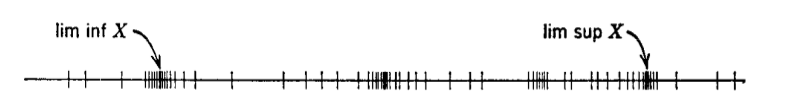
\includegraphics[height=1.5cm]{2_01.png}

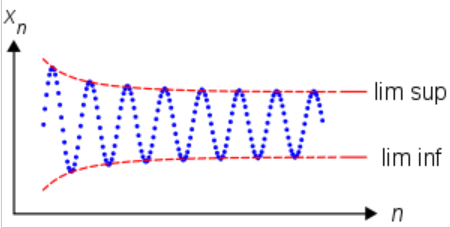
\includegraphics[height=3cm]{2_02.png}

Formel olarak diyelim ki $\{x_n\}$ bir seri, ve diyelim ki bir reel
sayi $S$ var, ki bu reel sayi su sartlari tatmin ediyor 
1) Her $\epsilon > 0$ icin bir $N$ var, oyle ki her $n>N$ icin $x_n
< S + \epsilon$ 
ve 2) her $\epsilon > 0$ ve $M>0$ icin bir  $n>M$ var ki $x_n
> S - \epsilon$. O 
zaman $S$ sayisina  $\{x_n\}$ serisinin limit superior'u denir. 

Bu tanimin soylemeye calistigi serinin yaklastigi degerden sonra ve once
sonlu buyuklukte (bir pencere tanimlarsak bu pencere icinde sonlu sayida
eleman olacaktir (sonsuz degil). Bu pencerenin tanimlanabiliyor olmasi,
onun makul bir noktada olmasini gerektirir, ki bu nokta da yaklasilan
degerden baskasi degildir. 

Limit inferior bunun tersidir, 

\[ \lim \inf x_n  = -\lim \sup(-x_n)\]





\end{document}
